%!TEX root = ResearchPlan_v2.tex

\section{Ethical issues}

There is no need of ethical considerations in any of the research done in ALICE experiment at the Large Hadron Collider in CERN.


\section{Implementation: schedule, budget, distribution of work} %%%%%%%%%%%%%%%%%%%%%%%%%%%%%%%
\label{sec:implementation}

Figure~\ref{fig:LHC-mid-term} shows the medium term running plan of the LHC. 
%%%%%%%%%% BEGIN FIGURE %%%%%%%%%%%%%%%%
\begin{figure}[htbp]
   \centering
   \resizebox{15cm}{!}{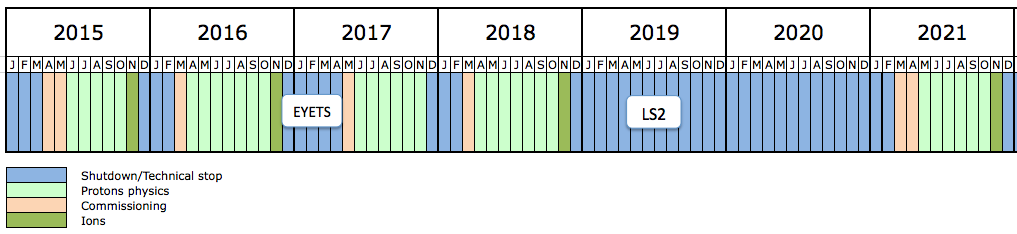
\includegraphics{LHC-medium-term.png}}
   \caption{Current draft of the medium term LHC running plan.}
   \label{fig:LHC-mid-term}
\end{figure}
%%%%%%%%%% END FIGURE %%%%%%%%%%%%%%%%%
We took lead-lead data in 2015 and will measure proton-lead at the end of 2016. After that there will be a longer end-of-the-year shutdown (EYETS). The purpose of the EYETS is to reduce workload that LHC would otherwise face during the Long Shutdown 2 (LS2) starting December 2018. Just before the LS2, there will be one more lead-lead campaign that ends the Run 2.

Year 2010 and 2011 heavy ion data (Run1) was taken at lower energy, $\sNN=2.76$~TeV, and 2015 data (Run2) with higher energy, $\sNN=5.02$~TeV. As ALICE reached the nominal design luminosity in 2015, that data set has 100 times more statistics compared to 2011 data set, that already was larger than 2010. However, we also experienced tracking problem in TPC due to accumulated space charge in high luminosity runs. It has turned out that calibration of 2015 data needs significantly more effort than earlier data sets. This may indicate that it will take substantial time in 2019 before 2018 heavy ion run results will be in hands of the analyzers. Due to these reasons, it may be that the 2015 heavy ion data will be the main source of data for analyzers that are promoted with this application. If LHC will not go to $\s{}=14$~TeV in proton-proton during Run 2, then for sure the 2018 heavy ion run will be with the same energy, $\sNN=5.02$~TeV. If all goes well, then both the 2015 and 2018 data sets are in good shape for physics analysis in beginning of 2020 and we should have significant statistics at hand.

Related to this application, currently our group is involved with completing of flow and jet analysis with Run1 and Run2 data. Two of our PhD students Jussi Viinikainen and Marton Vargyas are finishing analysis of jet fragmentation in p-Pb and Pb--Pb collisions. In September 2016, J. Viinikainen  presented his results in the parallel talk at the Hard Probes conference in Wuan, China. The first paper on correlations between magnitudes of two different flow harmonics is just accepted in Phys. Rev. Lett.~\cite{ALICE:2016kpq} and the manuscript was selected a PRL Editors' Suggestion. DongJo Kim was one of the main contributors for this paper in ALICE and he is the chair of the 2$^{\rm nd}$ paper which will contain higher order flow harmonics correlations as well as the transverse momentum and rapidity dependence of the correlations. This 2nd paper is currently being prepared for collaboration review and these results will be presented in the "Quark Matter 2017" conference in February 2017. 

%%%%%%%%%%%%%% TABLE : TimeTable for the analysis %%%%%%%%%%%
%\begin{table}[htdp]
\begin{table}[htp]
\caption{Rough timetable for expected milestones in the analysis.}
\begin{center}
\begin{tabular}{ L{1.6cm} | L{11.5cm} | L{1.0cm} }
Assigned & Task & Year \\
\hline
 & Reproducing flow observables from Run2 5TeV data &  2017 \\
PhD-     & Finishing the analysis on higher harmonic flow correlation  & 2018\\
student & Paper proposal from higher harmonic flow correlation & 2019 \\
 & Finishing paper and thesis on higher harmonic flow correlation & 2021 \\
 & PhD-studies (40 cr) and 6 months of Service Work (20 cr) &  \\
\hline
 & Charged hadron and jet $p_{T}$ spectra reconstruction & 2017 \\
 & Establishing hypothesis for various event section criteria of jets  & 2018 \\
Post doc & Systematic studies on for various event section criteria of jets & 2019 \\
 & Final paper for "Interplay of Hard and Soft Physics"  & 2021 \\
 & EMCal trigger maintenance & cont. \\
\hline
 Together& Systematic studies on flow observables for various event section criteria of jets & 2020 \\
\hline
\end{tabular}
\end{center}
\label{tab:timetable}
\end{table}
%%%%%%%%%%%%%% END TABLE %%% %%%%%%%%%%%

As the pre-requisites studies for correlations of flow harmonics from Run1 will be finalized in 2017, quite likely close to beginning of this application period, we will be in very good position to start the analysis outlined here. Table~\ref{tab:timetable} shows the outline we find realistic for studies that will combine current flow analysis to event selection bias coming from presence of hard jets.

One should note that the above is only for the analysis. Post doc will have to use fraction of his/her time for the EMCal trigger maintenance. PhD-student must give equivalent of total of 6 months of full working time to ALICE experiments service work. Regarding our obligations, the PhD student will be quite likely involved also in the TPC upgrade activities. The exact timing either to LS2 or preceding QA work will depend on the need. Our group members have to participate into our institutional share of the ALICE shift load during running of the experiment.

This applications has mainly salary and mobility allowances together with some travel costs which makes the budgeting in principle rather straightforward. We apply here a salary for a post doc and PhD-student positions, see Table~\ref{tab:money} for average yearly costs.
%%%%%%%%%%%%%% TABLE : MONEY %%%%%%%%%%%
\begin{table}[htp]
\caption{Main expenses in a yearly budget.}
\begin{center}
\begin{tabular}{l|l|r|r|r|r}
Position & Assignment & Salary & Mobility & Travel & Tot. cost\\
& & month & year & year & year \\\hline
Post doc & Analysis + EMCal running    & 3'350 & 12'600 & 2'000 & 116'762\\
PhD student & Analysis + TPC upgrade & 2'200 &  See text   & 2'000 & 69'090 \\
PI & Project leading & 6'000 &  See text   & See text & 22'870 \\
\multicolumn{5}{r}{Average full cost/year} & 208'722  \\
\end{tabular}
\end{center}
\label{tab:money}
\end{table}
%%%%%%%%%%%%%% END TABLE %%% %%%%%%%%%%%
As the post doc should be 100~\% of the time at CERN, due to planned responsibilities in EMCal running and maintenance, he/she would need (minimum) of $12\times1050$~\euro$/{\rm m}=12600$~\euro\ per year the mobility money. Also the PhD-student needs to spend significant time in CERN to perform the service work duties, do shifts and interact with Physics Working Group. Due to project size limitations, we could not embed his/her mobility costs to this application. We will use some other source, like annual HIP ALICE project resources, to this purpose.

Currently the post doc is not named, so this position would go into international call. Quite likely a suitable candidate could be a recently defended PhD inside the ALICE experiment, who has background in flow or EMCal jet analysis. He/she would then be very familiar with the experiment and analysis environment. Our group has a very good candidate to the PhD-student position, Jasper Parkkila. Jasper worked in our group in HIP's summer student program in 2016 and made very impressive student work when he participated to flow analysis that is going to published. Jasper is expected to finish his Master's Thesis in May-August 2017 so this project would provide him a secure funding for his PhD-thesis.

I would meet and supervise both post doc and PhD-student in CERN personally, as I spend a significant portion of the calendar year there all the time. In typical calendar year I am on-site at CERN roughly 6 months. I am also Finnish representative in ALICE collaboration board that requires presense at CERN, on top of the leading this project. Since I have also other duties on-site at CERN, my mobility expenses are covered by the direct funding that Ministry of Education provides to Finnish ALICE activities.

Also two senior members of the group, DongJo Kim and Sami R\"as\"anen, visit in CERN regularly and support the work of both. DongJo is a flow expert in our group and would be the co-supervisor in the PhD-students thesis work. Sami has a background in theory accompanied with significant teaching and student councelling experience, so he will make a contribution to steering of the analysis and how the results are related with theoretical studies.

\section{Research team and collaborative partners} %%%%%%%%%%%%%%%%%%%%%%%%%%%%%%%
\label{sec:reseachteam}

The Finnish involvement to ALICE experiment is carried out by the Department of Physics in University of Jyv\"askyl\"a (JYFL) and Helsinki Institute of Physics (HIP). At HIP the ALICE activities belong into the Nuclear Matter program coordinated by Ari Jokinen. Table~\ref{tab:personnel} shows the current members of ALICE analysis group in Jyv\"askyl\"a, the main persons involved in these activities, and their funding sources.

\begin{table}[htp]
\caption{ALICE-analysis group members in Jyv\"askyl\"a in September 2016.}
\begin{center}
\begin{tabular}{|l|l|l|l|l|}
\hline
   &  Name                       &  position         & Starting date & Funding \\
\hline
1 &    Jan  Rak                  & Professor       &  2005           & JYFL \\
2 &    DongJo   Kim          & Senior researcher     &  2006           & HIP \\
3 &    Sami   R\"as\"anen & Senior researcher     &  2008           & HIP \\
 \hline
4 &    Beomsu   Chang     & PhD student   &  Nov-11       & JYFL \\
5 &    Jussi   Viinikainen   & PhD student   & Jan-13         &  Ehrnrooth   \\
6 &    Tomas Snellman     & PhD student   & June-13       & HIP\\
7 &    Marton Vargyas      & PhD student   & Jan-14         & Vais\"al\"a\\
\hline
\end{tabular}
\end{center}
\label{tab:personnel}
\end{table}%

Besides the Jyv\"askyl\"a analysis group, we have two post doc's working in the HIP detector laboratory, Erik Brucken and Timo Hilden. Erik and Timo are working full time with the TPC upgrade. Other Finnish ALICE activities are pursued by senior researcher Wladyslaw Trzaska, who is leading the FIT project and professor Risto Orava who is leading ALICE-Forward group in HIP/Helsinki concentrating on diffractive physics.

Although CERN Physics Working Group (PWG) members are not directly involved with this project, they are providing invaluable support to the analysis work. Interaction of post doc and PhD-student with PWG will provide them substantial resource in guiding and making effective progress in the analysis work.

\section{Research careers, fulfillment of the mobility requirement and researcher training}%%%%%%%%%%%%%%%%%%%%%%%%%%%%%%%
\label{sec:career}

All the closest seniors in this project, the PI, DongJo Kim and Sami R\"as\"anen, clearly fulfill the Academy requirements for mobility. CERN research guarantees mobility automatically to all post doc's and PhD-students. Successful working in large high energy experiment also gives an excellent starting point to progress in career since young researches have chances to make themselves known while they work in CERN, which is one more justification to spend significant period of time on-site. ALICE collaboration has over 1500 members from 154 institutions and 37 countries. This opens up numerous possibilities to continue their academic career.

\section{Mobility plan}%%%%%%%%%%%%%%%%%%%%%%%%%%%%%%%
\label{sec:mobility}

As discussed in Sec.~\ref{sec:researchmethods}, we are responsible EMCal maintenance and operation and also participate into TPC ROC upgrade and FIT-detector design, building and commissioning. T0 and FIT activities are included into separate project application to Academy by Wladyslaw Trzaska. To fulfill the obligations related to EMCal and TPC activities, the hired post doc should be stationed at CERN all the time. Particularly the 2nd long shutdown after Run2, starting December 2018, will be busy time with the detector upgrades and maintenance. During the ongoing Run2, we need guarantee flawless running of the EMCal L0-trigger and provide regular trigger performance studies. This is the best achieved when the expert is on site.

The PhD-student would spend roughly 50~\% of his thesis project time at CERN. This would include analysis work in PWG and also equivivalent of 6 months of service work for the ALICE collaboration that is required from every PhD-student. The student would participate into TPC upgrade as his contribution.

Another important aspect of the research career in a big collaboration is that the place where the experiment is located is a natural place for meetings and it is also a place where majority of ``intellectual recourses'' can be found. Working on-site gives the best opportunity to make connections and become known inside the experiment.

\nopagebreak
